\documentclass[a4paper,11pt]{article}
%%%%%%%%%%%%%%%%%%%%%%%%%%%%%%%%%%%%%%%%%%%%%%%%%%%%%%%%%%%%%%%%%%%%%%%%%%%%%%%%
\usepackage{ccs_iogs}
%%%%%%%%%%%%%%%%%%%%%%%%%%%%%%%%%%%%%%%%%%%%%%%%%%%%%%%%%%%%%%%%%%%%%%%%%%%%%%%%
\begin{document}
\newpage
\begin{minipage}[c]{.25\linewidth}
	
\includegraphics[width=4cm]{images/LEnsE_IOGS.jpg}
\end{minipage} \hfill
\begin{minipage}[c]{.4\linewidth}

\begin{center}
\vspace{0.3cm}
{\Large OPTO-ELECTRONIQUE}

\medskip

\textbf{\Large TP Séance 6 / Filtre Num}

\end{center}
\end{minipage}\hfill

\begin{center}
\vspace{0.3cm}

\noindent \rule{\linewidth}{1pt}

Durée : 3h / Filtre Numérique

\vspace{-0.2cm}
\noindent \rule{\linewidth}{1pt}
\end{center}



%%%%%%%%%%%%%%%%%%%%%%%%%%%%%%%%%%
\section*{Objectifs de l'expérience}

On se propose dans ce TP d'étudier les caractéristiques d'un \textbf{filtre numérique} (Partie A) et d'un \textbf{filtre analogique} (Partie B), puis de réfléchir à l'intérêt de la mise en cascade de ces deux filtres.

%%%%%%%%%%%%%%%%%%%%%%%%%%%%%%%%%%

\section{PARTIE A - Filtre \textbf{Numérique} \textsc{\normalsize(Durée conseillée : 90 min)}}

On se propose d'étudier le \textbf{boitier annexe} fourni qui est un \textbf{système numérique}.

%%%%%%%%%%%%%%%%%%%%%%%%%%%%%%%%%%%%%%%%%%%%%
\noindent \rule{\linewidth}{1pt}

\textbf{\large \textsc{Attention : le boitier doit être alimenté entre 0 et 5V. Aucune tension négative n'est tolérée sur l'alimentation.}}

\textbf{\large \textsc{Les valeurs des tensions des signaux d'entrée devront être positives et inférieures à 3V.}}

\noindent \rule{\linewidth}{1pt}


\subsection*{A1 - Etude du mode SUIVEUR}

\Real Observer, en mode "SUIVEUR" (numérique), le comportement de ce système pour des signaux d'entrée de fréquence allant de 100Hz à 100kHz.


\Real Faire une analyse plus précise autour des valeurs de fréquence suivante: $f = 100 \, Hz$, $f = 1 \, kHz$, $f = 4 \, kHz$, $f = 20 \, kHz$ et $f = 25 \, kHz$. \textit{Il peut-être judicieux d'utiliser la \textbf{fonction FFT} de l'oscilloscope numérique.}

\Real Analyser les résultats obtenus et indiquer les valeurs numériques pertinentes caractérisant le fonctionnement de ce système.

\Real Préciser les limites de fonctionnement d'un tel système. Proposer une solution à mettre en oeuvre pour s'affranchir des problèmes liés à ces limites.

\subsection*{A2 - Etude du mode FILTRE}

\Real Proposer un protocole pour caractériser en fréquence ce système.

\textit{On fera l'hypothèse que le mode FILTRE est soumis aux mêmes limites que le mode SUIVEUR.}

\Real Caractériser ce système en fréquence. 

\Real Justifier le choix de l'intervalle de fréquences testées.

\Real Analyser vos résultats pour valider le comportement de ce filtre.


%%%%%%%%%%%%%%%%%%%%%%%%%%%%%%%%%%

\newpage
%%%%%%%%%%%%%%%%%%%%%%%%%%%%%%%%%%
%%%%%%%%%%%%%%%%%%%%%%%%%%%%%%%%%%
%%%%%%%%%%%%%%%%%%%%%%%%%%%%%%%%%%

\section{PARTIE B - Filtre anti-repliement analogique \textsc{\normalsize(Durée conseillée : 90 min)}}


On se propose d'étudier un filtre actif basé sur une structure de Rauch (la pulsation caractéristique de ce filtre est donnée ci-dessous).

\begin{center}
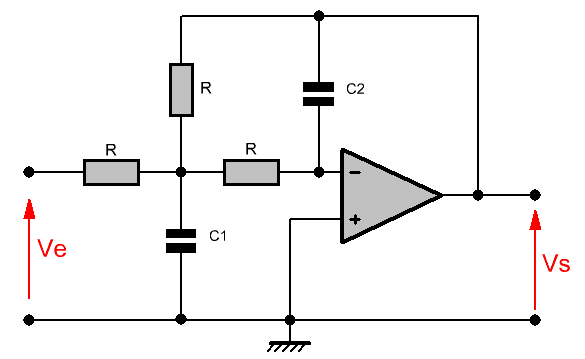
\includegraphics[scale=0.8]{images/rauch.png}
\end{center}

La pulsation caractéristique de ce filtre vaut $\omega_c = \frac{1}{R \cdot \sqrt{C_1 C_2}}$ et le facteur de qualité vaut $Q = \frac{1}{3} \cdot \sqrt{\frac{C_1}{C_2}}$.

%
%%%%%%%%%%%%%%%%%%%%%%%%%%%%%%%%%%
\subsection*{B1 - Etude théorique}


Ce montage utilise un amplificateur linéaire intégré (ALI) de type \texttt{TL071} (voir documentation en annexe) qui fonctionne ici en régime linéaire. On a alors la relation suivante sur les entrées de l'ALI : $V+ = V-$ et les courants d'entrée $i+$ et $i-$ de cet amplificateur sont supposés nuls.

\Real Faire une étude du fonctionnement du circuit en basse et en haute fréquence. En déduire le comportement attendu de ce filtre et donner les valeurs numérique le caractérisant pour les valeurs de composants suivantes: $R = 2.2~k\Omega$, $C_1 = 22~nF$, $C_2 = 2.2~nF$. 

%%%%%%%%%%%%%%%%%%%%%%%%%%%%%%%%%%
\subsection*{B2 - Alimentation symétrique}
\parpic[r]{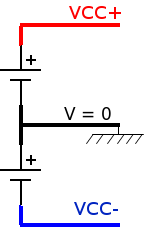
\includegraphics{images/Alim_cablageVCC.png}}

\Real Réaliser une alimentation symétrique de +$V_{CC}$ / -$V_{CC}$ (avec $V_{CC} = 5~V$) à l'aide de l'alimentation continue composée de deux blocs indépendants (voir document annexe \textit{Description du matériel} et figure ci-contre).

\Real Proposer et mettre en oeuvre une méthode de validation de ces deux tensions (successivement).



%%%%%%%%%%%%%%%%%%%%%%%%%%%%%%%%%%%%%%%%%%%%%
\noindent \rule{\linewidth}{1pt}

\textbf{\large \textsc{Attention : les signaux d'entrée ne pourront pas dépasser les tensions d'alimentation et seront donc contraints à des amplitudes inférieures à $V_{CC}$}}	

%%%%%%%%%%%%%%%%%%%%%%%%%%%%%%%%%%
\subsection*{B3 - Etude en fréquence de cette structure}

\Real Réaliser le montage précédent avec les valeurs de composants $R = 2.2~k\Omega$, $C_1 = 22~nF$, $C_2 = 2.2~nF$. 

\Real Proposer un protocole d'étude en fréquence de ce montage.

\Real Caractériser ce système pour des fréquences allant de 10Hz à 100kHz.

\Real Analyser les résultats pour valider le comportement de ce filtre.


\subsection*{B4 - Mise en cascade des montages}

\Real Expliquer l'intérêt de mettre en cascade ce montage avec celui de la partie précédente.

\Real Mettre en \oe{}uvre cette mise en cascade et vérifier l'impact sur l'atténuation des problèmes identifiés dans la partie A.


%%%%%%%%%%%%%%%%%%%%%%%%%%%%%%%%%%%%%%%%%%%%%%%%%%%%%%%%%%%%%%%%%%%%%%%%%%%%%%%%%%%%%
\end{document}
